g% --- Template for thesis / report with tktltiki2 class ---

\documentclass[finnish]{tktltiki2}

% tktltiki2 automatically loads babel, so you can simply
% give the language parameter (e.g. finnish, swedish, english, british) as
% a parameter for the class: \documentclass[finnish]{tktltiki2}.
% The information on title and abstract is generated automatically depending on
% the language, see below if you need to change any of these manually.
% 
% Class options:
% - grading                 -- Print labels for grading information on the front page.
% - disablelastpagecounter  -- Disables the automatic generation of page number information
%                              in the abstract. See also \numberofpagesinformation{} command below.
%
% The class also respects the following options of article class:
%   10pt, 11pt, 12pt, final, draft, oneside, twoside,
%   openright, openany, onecolumn, twocolumn, leqno, fleqn
%
% The default font size is 11pt. The paper size used is A4, other sizes are not supported.
%
% rubber: module pdftex

% --- General packages ---

\usepackage[utf8]{inputenc}
\usepackage{lmodern}
\usepackage{microtype}
\usepackage{amsfonts,amsmath,amssymb,amsthm,booktabs,color,enumitem,graphicx}
\usepackage[pdftex,hidelinks]{hyperref}

% Automatically set the PDF metadata fields
\makeatletter
\AtBeginDocument{\hypersetup{pdftitle = {\@title}, pdfauthor = {\@author}}}
\makeatother

% --- Language-related settings ---
%
% these should be modified according to your language

% babelbib for non-english bibliography using bibtex
\usepackage[fixlanguage]{babelbib}
\selectbiblanguage{finnish}

% add bibliography to the table of contents
\usepackage[nottoc,numbib]{tocbibind}
% tocbibind renames the bibliography, use the following to change it back
\settocbibname{Lähteet}

% --- Theorem environment definitions ---

\newtheorem{lau}{Lause}
\newtheorem{lem}[lau]{Lemma}
\newtheorem{kor}[lau]{Korollaari}

\theoremstyle{definition}
\newtheorem{maar}[lau]{Määritelmä}
\newtheorem{ong}{Ongelma}
\newtheorem{alg}[lau]{Algoritmi}
\newtheorem{esim}[lau]{Esimerkki}

\theoremstyle{remark}
\newtheorem*{huom}{Huomautus}


% --- tktltiki2 options ---
%
% The following commands define the information used to generate title and
% abstract pages. The following entries should be always specified:

\title{Ketterien menetelmien tarjoamia ratkaisuja suunnitelmavetoisten prosessimallien ongelmiin}
\author{Jarl-Erik Malmström}
\date{\today}
\level{Kandidaatintutkielma}
\abstract{Tiivistelmä.}

% The following can be used to specify keywords and classification of the paper:

\keywords{agile, ketterä, iteraatiivinen, inkrementaalinen, ohjelmistotuotantomenetelmät}
\classification{} % classification according to ACM Computing Classification System (http://www.acm.org/about/class/)
                  % This is probably mostly relevant for computer scientists

% If the automatic page number counting is not working as desired in your case,
% uncomment the following to manually set the number of pages displayed in the abstract page:
%
% \numberofpagesinformation{16 sivua + 10 sivua liitteissä}
%
% If you are not a computer scientist, you will want to uncomment the following by hand and specify
% your department, faculty and subject by hand:
%
% \faculty{Matemaattis-luonnontieteellinen}
% \department{Tietojenkäsittelytieteen laitos}
% \subject{Tietojenkäsittelytiede}
%
% If you are not from the University of Helsinki, then you will most likely want to set these also:
%
% \university{Helsingin Yliopisto}
% \universitylong{HELSINGIN YLIOPISTO --- HELSINGFORS UNIVERSITET --- UNIVERSITY OF HELSINKI} % displayed on the top of the abstract page
% \city{Helsinki}
%


\begin{document}

% --- Front matter ---

\maketitle        % title page
\makeabstract     % abstract page

\tableofcontents  % table of contents
\newpage          % clear page after the table of contents


% --- Main matter ---

\section{Johdanto}
 
Ohjelmistotuotannossa (software engineering) käytetään työn suunnitteluun ja organisointiin ohjelmistotuotantomenetelmiä (software development methodologies). Menetelmät määrittelevät formaalin prosessin, jonka lopputuloksena valmistuu toimiva ohjelmisto. Ohjelmistotuotannon menetelmät ovat olleet käytössä pitkään. Ohjelmistojen parissa työskentelevät olivat muiden alojen insinöörejä ja matemaatikkoja ja menetelmät olivat omaksuttu muista insinööritieteistä. Tietokoneet olivat kookkaita sekä käyttökustannukset olivat ohjelmistoja tuottavien insinöörien palkkoihin verrattuna korkeat. Koska ohjelmistojen suorittaminen tietokoneilla oli kallista, ohjelmistokehitys vaati tiukkaa suunnittelua sekä järjestelmällisiä käytäntöjä\cite{BOE06}.   

Menetelmät toivat ohjelmistokehitykseen ennakoitavuutta ja tehokkuutta. Muista insinööritieteistä vaikutteita saaneet menetelmät olivat yksityiskohtaisia prosesseja, joissa painotettiin voimakkaasti dokumentointia, määrittelyä ja suunnittelua, jotka tuli toteuttaa ennen ohjelmiston toteutusta\cite{FOW01a}.

Vuoteen 1960 mennessä ohjelmistojen parissa toimiville ihmisille alkoi selvitä, että ohjelmiston kehitykseen liittyvät ilmiöt poikkesivat huomattavasti laitteistoihin liittyvistä ilmiöistä. Ohjelmistoja oli paljon helpompi muuttaa kuin laitteistoja eikä ohjelmistojen kopioiminen vaatinut kalliita tuotantolinjoja. Ohjelmistojen helppo muokattavuus sai monet ihmiset ja organisaatiot omaksumaan \textit{ohjelmoi ja korjaa} (\textit{code and fix}) menetelmän\cite{BOE06}.

Reaktiona 1960-luvun \textit{ohjelmoi ja korjaa} lähestymistapaan, laadittiin menetelmiä, mitkä olivat tarkemmin organisoituja. Menetelmissä varsinaista ohjelmointia edelsi tarkka vaatimusmäärittely ja suunnitteluvaihe\cite{BOE06}.

Ohjelmistojen hankintasopimukset asettivat ohjelmistotuotannon menetelmille selkeät vaatimukset. Yhdysvaltain hallituksen ja puolustusministeriön vaatimien ohjelmistotuotantomenetelmien tuli koostua peräkkäisistä prosesseista. Suunnittelua ei aloitettu ennen kuin ohjelmiston vaatimukset oli täydellisesti kirjattu. Eikä ohjelmointia aloitettu ennen suunnitelman tyhjentävää ja kriittistä tarkastelua. Yhdysvaltain hallituksen luomat standardit prosesseille aiheuttivat tulkinnan, että ohjelmistotuotantomenetelmien täytyy olla vaiheesta seuraavaan etenevä lineaarinen prosessi\cite{BOE06}.

Winston Roycen artikkelissa ''Managing the Development of Large Software Systems'' esittämiä ajatuksia pidetään vesiputousmallin (waterfall model) perustana. Vesiputousmalli vastasi valtionhallinnon sopimusten vaatimuksiin\cite{LAB03}.

Uusia menetelmiä on kehitetty vesiputousmallin mukaisille suunnittelua ja dokumentaatiota painottavien menetelmien tilalle. Näitä kutsutaan yleisesti ketteriksi menetelmiksi (agile methods). Ketterät menetelmät ovat olleet reaktio byrokraattisille ja raskaille menetelmille. Ketterät menetelmät pyrkivät kompromissiin, \textit{ohjelmoi ja korjaa}-menetelmän ja raskaan menetelmän väliltä, tarjoamalla riittävän prosessin haluttuun lopputulokseen pääsemiseksi\cite{FOW01a}. Ketterät menetelmissä painotetaan ihmisiä sekä heidän välistä viestintää.  Menetelmissä asetetaan luottamus ihmisten taitoon ja lahjakkuuteen

Tässä tutkielmassa tarkastelemme ohjelmistotuotannon suunnitelmavetoisten prosessimallien ongelmia. Käymme läpi erilaisia dokumentti- ja suunnitelmavetoisia menetelmiä sekä niiden lähestymistapoja ohjelmistotuotantoon. Nykyisin vesiputousmallin mukaisia suunnitelmavetoisia menetelmiä kritisoidaan raskaiksi ja byrokraattisiksi. Menetelmien määrittely- ja suunnitteluvaihe sekä dokumentoinnin painotus hidastavat ohjelmistotuotantoprosessia ohjelmistotuotannossa, jossa vaatimukset muuttuvat\cite{FOW01a}. Tarkastelemme miten ketterät menetelmät (agile methods) ovat pyrkineet ratkaisemaan raskaan suunnitteluvaiheen sisältävien prosessimallien heikkouksia.

\section{Ohjelmistotuotannon ongelmat}

Kunnianhimoisin tietojenkäsittelyntieteen projekti 1950-luvulla oli SAGE-järjestelmä (Semi-Automated Ground Environment) Yhdysvaltojen ja Kanadan puolustusvoimille. Projekti kokosi yhteen tutka-, viestintä- ja tietokoneinsinöörejä sekä myös ensimmäisiä ohjelmistoinsinöörejä. Ohjelmiston tuotannossa käytettävä menetelmä oli vaiheesta seuraavaan etenevä lineaarinen prosessi. Vaatimukset täyttävä ohjelmisto valmistui vuoden aikataulusta myöhässä. Ohjelmistoprojektin koettiin myöhästymisestä huolimatta onnistuneen, ja suurimpana onnistumiseen vaikuttavana tekijänä nähtiin insinööritieteistä omaksutut käytänteet\cite{BOE06}.

Ohjelmistot merkityksen kasvaessa ihmisten ja tietokoneiden vuorovaikutus korostui yhä enemmän. Tietokonelaitteistojen merkitys väheni. Monet ohjelmistotuotantoprojektit vaativat yhä enemmän ihmisiä tuottavaan ja luovaan työhön. Muista insinööritieteistä omaksutuilla menetelmillä ei voitu arvioida ohjelmistojen luotettavuutta kattavasti. Ohjelmistotuotannon kustannukset alkoivat kasvaa. Ohjelmistoprojektien aikatauluja oli vaikea ennakoida, ja henkilöstön lisääminen aikataulun nopeuttamiseksi saattoi myöhästyttää projektia entisestään\cite{BOE06}.

Ohjelmistotuotantoon tarvittiin enemmän insinöörejä ja matemaatikkoja kuin oli saatavilla. Ohjelmistotuotantoprojekteihin palkattiin yhä enemmän myös muiden alojen asiantuntijoita, jotka omaksuivat helposti ''ohjelmoi ja korjaa''-käytännöt insinöörimenetelmien sijasta. Suuri ero perinteisten insinöörimenetelmien ja ''ohjelmoi ja korjaa'' asenteen välillä loi uutta ''hakkeri kulttuuria'' merkittävien yliopistojen tietojenkäsittelylaitoksille. Nämä auktoriteetteja vastustavat luovat ''sankari ohjelmoijat'' tekivät usein vaikeasti muutettavaa ja ylläpidettävää ohjelmakoodia\cite{BOE06}.

Ennen 1960-luvun loppua NATO:n tiedekomitea järjesti kaksi ohjelmistotekniikan (software engineering) suurta konferenssia, johon osallistui monia alan ammattilaisia ja johtavia tutkijoita. Nämä konferenssit loivat vahvan pohjan ohjelmistotekniikalle ja -tuotannolle, joita teollisuus ja julkishallinnon organisaatiot käyttivät perustana vaatimuksilleen ohjelmistotuotantoprojekteissa käytettävistä menetelmistä. Oli selvää, että tarvit\-tiin organisoituja ja kurinalaisia käytäntöjä yhä suuremmille projekteille ja tuotteille\cite{BOE06}.

Ohjelmakoodia kirjoitettiin usein ilman taustalla olevaa suunnitelmaa. Tällainen menetelmä saattaa toimia jos tuotettava ohjelmisto on pieni, mutta järjestelmän kasvaessa uusien toiminnallisuuksien lisääminen vaikeutuu. Lisäksi virheiden korjaaminen vaikeutuu järjestelmän kasvaessa\cite{FOW01a}.

\subsection{Koordinointi}

Onnistunut ohjelmistojärjestelmä vaatii erilaisten pyrkimysten koordinointia ohjelmistokehityksen aikana. Ohjelmistojärjestelmien perustavanlaatuinen ominaisuus on niiden suuri koko. Yksilöiden tai pienten ryhmien on mahdotonta luoda tai ymmärtää suuria ohjelmistoja yksityiskohtaisesti\cite{KES95}.

Ohjelmistolla on yleensä paljon erilaisia ohjelmakoodin polkuja (path), jotka johtavat erilaisiin tiloihin (state). Tämä tekee tietojen määrittelystä (specification) ja ohjelmiston testaamisesta vaikeaa\cite{BOE06}.

Suuret projektit onnistuvat useimmin jos projektia koordinoi henkilö, jolla on tietoa ohjelmiston toimialalta sekä ohjelmistoalalta\cite{KES95}.

Tällainen ideaalitilanne on usein mahdotonta suurille ohjelmistojärjestelmille, joiden koko voi olla miljoonia tai kymmeniä miljoonia ohjelmarivejä sekä projektin kesto useita vuosia\cite{KES95}.

Suuren kokoluokan pyrkimykset johtavat erikoistumiseen ja työn jakamiseen. Organisaatiossa tämä johtaa toisistaan riippuvien tekijöiden jakamiseen osastoihin maantieteellisesti, organisatorisesti, sekä sosiaalisesti. Tämä vähentää mahdollisuuksia ja haluja oppia sekä jakaa tietoa etäisten työtovereiden kesken\cite{KES95}.

Ohjelmistotuotannon luontainen epävarmuus lisää koordinointiongelmaa. Toisin kuin teollinen valmistus, ohjelmistokehitys ei ole rutiininomainen toimi. Monet ohjelmistojärjestelmät ovat yksilöllisiä projekteja, ilman olemassa olevaa prototyyppiä, tai muokattavaa ohjelmistoa\cite{KES95}.

\subsection{Muuttuvat vaatimukset}

Lisäksi epävarmuus lisääntyy, koska ohjelmiston toimintaan liittyvät vaatimukset muuttuvat\cite{KES95}.

Muutoksia ohjelmiston vaatimuksiin esiintyy, koska ympäristö mihin ohjelmisto suunniteltiin muuttuu. Liiketoiminta, käyttäjien toiveet, tietokoneympäristö, ohjelmiston syötteet ja fyysinen maailma itsessään muuttuvat\cite{KES95}.

Muutostarpeiden ilmaantumisen todennäköisyys on suurin ohjelmistoa käytettäessä. Tällöin käyttäjät usein ymmärtävät ohjelmiston rajoitteet ja mahdollisuudet. Kun ohjelmistoa käytetään olosuhteissa, johon sitä ei ollut alunperin kuviteltu alkuperäistä suunnitelmaa tehtäessä, niin käyttäjät todennäköisesti vaativat uusia toiminnallisuuksia\cite{KES95}.

Ohjelmistokehitys on epävarmaa, koska vaatimukset ovat poikkeuksetta epätäydellisiä. Epätäydellisyys aiheutuu osittain rajallisista toimialan tiedoista ja ohjelmistoprojektin tyypillisestä työn jakamisesta. Liian vähällä, projektissa työskentelevillä ihmisillä, on riittävää tuntemusta toimialasta\cite{KES95}.

Ohjelmistojen vaatimusten muuttuminen projektin edetessä ei ole ohjelmistotuotannossa kuitenkaan uusi ongelma. Royce vuonna 1970 ja Boehm vuonna 1988 artikkeleissaan\cite{ROY70}\cite{BOE88} käsittelivät ohjelmistokehityksen muuttuvaa luonnetta. 

Avaruussukkulajärjestelmän kehityksessä 70-ja 80-luvulla, aikaisempien kokemuksien perusteella, NASA ja IBM osasivat odottaa muuttuvia vaatimuksia\cite{MWR84}. Sukkulaohjelman ohjelmistokehityksessä muun muassa seuraavat tavoitteet otettiin huomioon: 

\begin{itemize}
 \item Toteutetaan ensimmäiseksi kehittyneimmät vaatimukset
 \item Maksimaalisen testauksen varmistamiseksi julkaistaan ohjelmistoa mahdollisimman nopeasti\cite{MWR84}.
\end{itemize}

Tyypillisesti analyytikko vaihtelevalla toimialan tuntemuksella haastattelee asiakkaita ja käyttäjiä. Tämän jälkeen analyytikko kirjoittaa vaatimukset ohjelmistoarkkitehdeille ja -suunnittelijoille. Tässä prosessissa merkityksellistä toimialatietoa poikkeuksetta katoaa\cite{KES95}.

Kaikkia käyttäjien tarpeita analyytikko ei löydä ja jotkin tarpeet jäävät kirjaamatta vaatimusmäärittelyyn. Suuri koordinointiongelma ohjelmistokehityksessä on, että ohjelmistoarkkitehtien ja -suunnittelijoiden päätöksentekoon tarvitsema tieto ei ole saatavilla käytettävissä olevissa dokumenteissa\cite{KES95}.

Suuri kokoluokka ja epävarmuus olisivat vähäisempiä ongelmia, jos ohjelmisto ei vaatisi sen osajärjestelmien täsmällistä integraatiota. Ohjelmistot pääasiallisesti ovat rakennettu useista osista, jotka on kytkettävä yhteen, jotta ohjelmisto toimisi oikein\cite{KES95}.

\subsection{Liiketoimintaympäristö ja internet}

Liiketoimintaympäristö muuttuu nykyisin nopeassa tahdissa. Teknologian ja liiketoiminnan vaatimusten muuttuessa tehdyt vaatimusmäärittelyt ja suunnitelmat vanhentuvat nopeasti\cite{WIC03}. Alkuperäisen vaatimusmäärittelyn ja suunnitelman seuraaminen ei ole ohjelmistoprojektien pääasiallinen päämäärä. Sen sijaan toimitettavan ohjelmiston tarkoitus on asiakkaan, mahdollisesti vaihtuvien, tarpeiden tyydyttäminen\cite{HIC01}.

Internet liiketoimintaympäristönä vahvistaa ohjelmistotuotannon ongelmia korostamalla nopeutta. Asiakkaat vaativat liiketoiminnalle arvoa tuottavia ominaisuuksia nopeammassa tahdissa kuin koskaan aikaisemmin\cite{BRL03}.

\subsection{Tekninen kehitys}


Käytännön kokemus osoittaa, että aikaisempi ohjelmistotuotannon kehitys ei ole onnistunut ratkaisemaan suurien ohjelmistoprojektien koordinointiongelmia. 
Voidaan sanoa, että aikaisemmat ehdotetut korjaustoimenpiteet ovat lähestyneet ongelmaa seuraavasti: 
\begin{itemize}
 \item Tekniset työkalut, kuten tekstimuokkain (editor) tai korkean tason kielet
 \item Ohjelmiston jakaminen osiin (modularization) teknisesti, esimerkiksi olio-ohjelmoinnilla (object-oriented programming). Tai hallinnollisesti vaatimusmäärittelyn, ohjelmoinnin ja testaus toimintojen eriyttämisellä.
 \item Teknisillä formaaleilla menettelytavoilla, esimerkiksi versionhallinta, testisuunnitelma ja vaatimusmäärittelydokumentit\cite{KES95}.
\end{itemize}

\subsection{Ohjelmistotuotannon riskit}

Barry Boehm artikkelissaan ''A spiral model of software development and enhancement'' listaa ohjelmistotuotannon 10 suurinta riskiä: 

\begin{enumerate}
  \item Henkilöstö vaje.
  \item Epärealistinen aikataulu ja budjetti.
  \item Väärien ohjelmiston toiminnallisuuksien kehitys.
  \item Vääränlaisen käyttöliittymän kehitys.
  \item Ohjelmiston ominaisuuksien parantelu vaatimusten täytyttyä.
  \item Jatkuvasti vaihtuvat vaatimukset.
  \item Puutteet ulkoisesti toimitetuissa ohjelmiston osissa.
  \item Puutteet ulkoisesti suoritetuissa tehtävissä.
  \item Puutteet reaaliaikaisuuden suorituskyvyssä.
  \item Tietojenkäsittelytieteen valmiuksien ylikuormitus\cite{BOE88}.
\end{enumerate}

\section{Suunnitelmavetoiset menetelmät}

\subsection{Vesiputousmalli}

Ohjelmistotuotannossa on kaksi perustavanlaatuista vaihetta: analysointivaihe ja rakennusvaihe. Nämä kaksi vaihetta riittävät ohjelmiston toteuttamiseen jos ohjelmisto on pieni ja tuotettavan ohjelmiston käyttäjät ovat itse toteuttajia. Vaiheet pitävät sisällään aidosti luovaa työtä, joka suoraan edistää tuotettavaa ohjelmistoa\cite{ROY70}.

Suuremman ohjelmistotuotantoprojektin täytäntöönpano vaatii lisäksi muita vaiheita, jotka eivät suoraan edistä tuotettavaa ohjelmistoa ja lisäksi kasvattavat ohjelmistotuotannon kustannuksia\cite{ROY70}.

Ohjelmistotuotannon alkuaikoina käytetty ''ohjelmoi ja korjaa''-mallin sisältää kaksi vaihetta. Ohjelmoidaan ensin ja mietitään vaatimuksia, rakennetta sekä testausta myöhemmin. Mallilla oli useita heikkouksia. Usean korjausvaiheen jälkeen ohjelmakoodi oli niin vaikeasti rakennettu, että oli hyvin kallista muuttaa koodia. Tämä korosti tarvetta suunnitteluvaiheelle ennen ohjelmointia\cite{BOE88}.

Usein hyvin suunniteltu ohjelmisto ei vastannut käyttäjien toiveita. Joten syntyi tarve vaatimusmäärittelylle ennen suunnitteluvaihetta\cite{BOE88}. 

Ohjelmistot olivat usein kalliita korjata, koska muutoksiin ja testaamiseen oli valmistauduttu huonosti. Tämä osoitti tarpeen eri vaiheiden tunnistamiselle, sekä tarpeen huomioida testaus ja ohjelmiston muuttuminen jo hyvin varhaisessa vaiheessa\cite{BOE88}. 

1970-luvulla vesiputousmalli vaikutti suuresti lineaarisiin ohjelmistotuotannon malleihin. Vesiputousmallin lähestymistapa auttoi poistamaan monia aiemmin ohjelmistotuotantoa vaivanneita ongelmia. Vesiputousmallista tuli perusta monille teollisuuden ja Yhdysvaltain hallituksen ohjelmistohankintojen standardeille\cite{BOE88}.

Monet pitävät virheellisesti Roycen artikkelia lineaarisen menetelmän esikuvana. Roycen artikkelin iteratiivinen ja palautteen ohjaama ohjelmistokehitys, jossa ohjelmisto toteutetaan kahdesti, on unohtunut useista menetelmän kuvauksista\cite{LAB03}.

Tarkemmin Winston W. Roycen malli sisältää seuraavat vaiheet: järjestelmä- ja ohjelmistovaatimusmäärittely, analyysi, ohjelmistonrakenteen suunnittelu, ohjelmointi, testaus ja ohjelmiston käyttäminen\cite{ROY70}. 

Perättäisten ohjelmistotuotantovaiheiden välillä on iteraatiota järjestelmän rakenteen tarkentuessa yksityiskohtaisemmaksi tuotannon edetessä. Iteraatioiden tarkoituksena on suunnitelman edetessä pitää muutosvauhti käsiteltävän kokoisena\cite{ROY70}.

\subsection{Vesiputousmallin vaiheet}

Kuvassa 1. on yleisin kuvaus lineaarisesta vesiputousmallista. Roycen kuvaama prosessi, tässä yksinkertaisessa muodossa, oli tarkoitettu vain suoraviivaisimmille projekteille. Royce oli iteratiivisten, inkrementaalisten ja kehityksellisten (evolutionary) menetelmien kannattaja. Artikkelissa “Managing the Development of Large Software Systems”, 1960-1970 lukujen Yhdysvaltain hallituksen sopimusten vaatimat rajoitteet huomioiden, Royce kuvaa ohjelmistotuotannon iteratiivista prosessia\cite{LAB03}. 

\begin{figure}[h!]
  \caption{Lineaarinen ohjelmistotuotantoprosessi}
  \centering
    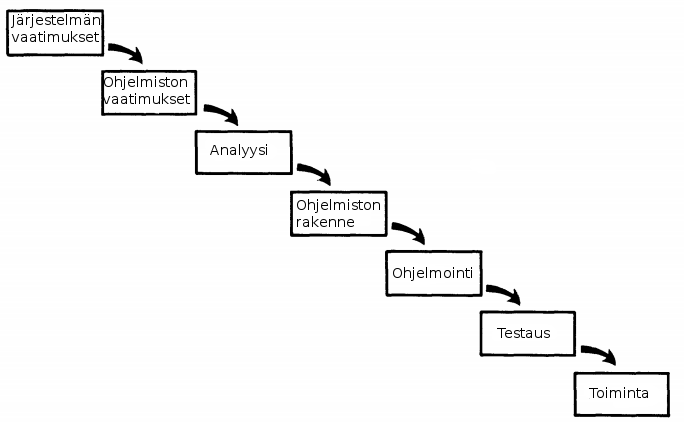
\includegraphics[width=\textwidth]{waterfall}
\end{figure}

\subsection*{Järjestelmän ja ohjelmiston vaatimukset}
Tässä vaiheessa kehitettävän järjestelmän ja ohjelmiston kaikki mahdolliset vaatimukset ja rajoitteet tuodaan esiin. Vaatimukset ovat joukko toiminnallisuuksia joita loppukäyttäjä odottaa ohjelmistolta. Järjestelmän ja laitteiston asettamat rajoitteet ohjelmiston suorituskyvylle on otettava huomioon.

\subsection*{Analyysi}
Ennen ohjelmiston rakenteen suunnittelua vaatimukset ovat analysoitava. Vaatimukset selvitetään loppukäyttäjältä ohjelmistokehityksen alussa. Loppukäyttäjien vaatimuksien ja liiketoimintaympäristön analysointi on edellytys ohjelmiston rakenteen suunnittelulle.  

 \subsection*{Ohjelmiston rakenne}
Ohjelmiston rakenteen suunnittelussa on otettava huomioon ohjelmiston erilaisten osien yhteensopivuus, ohjelmiston arkkitehtuuri ja erilaisten luokkien rakenne ja toiminnallisuus.  

 \subsection*{Ohjelmointi}
Ohjelmoijat kirjoittavat ohjelmiston ohjelmakoodin suunnitelmien perusteella.

 \subsection*{Testaus}
Testaajat varmistavat, että ohjelmisto toimii vaatimusten mukaan. Royce kirjoittaa, että testauksen tulisi tehdä siihen erikoistuneet henkilöt, jotka eivät välttämättä ohjelmoineet itse alkuperäistä ohjelmiston osaa. Royce painottaa dokumentin tärkeyttä, jotta testaaja voisi ymmärtää ohjelmiston toimintaa\cite{ROY70}. Useimmat virheet ovat luonteeltaan ilmiselviä, jotka voidaan löytää visuaalisella tarkastelulla. Jokaisen analyysin ja ohjelmakoodin tulee tarkastaa toinen henkilö, joka ei osallistunut varsinaiseen työhön. Jokainen tietokoneohjelman looginen polku on testattava ainakin kerran\cite{ROY70}.

 \subsection*{Toiminta}
Ohjelmiston operatiivinen käyttö.

\subsection*{Lineaarisen mallin riskit}

Royce huomioi lineearisen ohjelmistotuotantoprosessin sisältämän huomattavan riskin. Vasta testivaiheessa, menetelmän loppupuolella, saattaa tulla esille ilmiöitä, joita ei ollut mahdollista tarkalleen analysoida aikaisemmassa vaiheessa. Ellei pieni muutos koodissa korjaa ohjelmistoa vastaamaan oletettua käytöstä, vaadittavat muutokset ohjelmiston rakenteeseen saattavat olla niin häiritseviä, että muutokset rikkovat ohjelmistolle asetettuja vaatimuksia. Tällöin joko vaatimuksia tai suunnitelmaa on muutettava. Tässä tapauksessa tuotantoprosessi on palannut alkuun ja kustannusten voidaan olettaa nousevan jopa 100\%\cite{ROY70}.

Ongelman korjaamiseksi vaatimusmäärittelyn jälkeen - ennen analyysia - on tehtävä alustava rakenteen suunnittelu. Näin ohjelmistosuunnittelija välttää tallentamiseen tai aika -ja tilavaatimuksiin liittyvät virheet. Analyysin edetessä ohjelmistosuunnittelijan on välitettävä aika- ja tilavaatimukset sekä operatiiviset rajoitteet analyysin tekijälle\cite{ROY70}.

Näin voidaan tunnistaa projektille varatut alimitoitetut kokonaisresurssit tai virheelliset operatiiviset vaatimukset aikaisessa vaiheessa. Vaatimukset ja alustava suunnitelma voidaan iteroida ennen lopullista suunnitelmaa, ohjelmointia ja testausvaihetta\cite{ROY70}.

\subsection*{Dokumentointi}

Artikkelissaan Royce painottaa kattavan dokumentoinnin tärkeyttä: On laadittava ymmärrettävä, valaiseva ja ajantasainen dokumentti, jonka jokaisen työntekijän on sisäistettävä. Vähintään yhden työntekijällä on oltava syvällinen ymmärrys koko järjestelmästä, mikä on osaltaan saavutettavissa dokumentin laadinnalla\cite{ROY70}.

Ohjelmistosuunnittelijoiden on kommunikoitava rajapintojen(interface) suunnittelijoiden, ja johdon kanssa. Dokumentti antaa ymmärrettävän perustan rajapintojen suunnitteluun ja hallinnollisiin ratkaisuihin. Kirjallinen kuvaus pakottaa ohjelmistosuunnittelijan yksiselitteiseen ratkaisuun ja tarjoaa konkreettisen todistuksen työn valmistumisesta\cite{ROY70}.

Hyvän dokumentoinnin todellinen arvo ilmenee tuotannossa myöhemmin testausvaiheessa, ohjelmistoa käytettäessä sekä uudelleen suunniteltaessa. Hyvän dokumentin avulla esimies voi keskittää henkilöstön ohjelmistossa ilmenneisiin virheisiin. Ilman hyvää dokumenttia, ainoastaan ohjelmistovirheen alkuperäinen tekijä kykenee analysoimaan kyseessä olevan virheen\cite{ROY70}.

Dokumentti helpottaa ohjelmiston käyttöönottoa operatiivinen henkilöstön kanssa. Käyttöönotossa ilmenneiden mahdollisten ohjelmistovirheiden korjaamisessa selkeä dokumentti on välttämätön\cite{ROY70}.

\subsection*{Prototyyppi}

Dokumentoinnin jälkeen toinen ohjelmistoprojektin onnistumiseen vaikuttava tärkein tekijä on ohjelmiston alkuperäisyys. Jos kyseessä olevaa ohjelmistoa kehitetään ensimmäistä kertaa, on asiakkaalle toimitettava käyttöönotettava versio oltava toinen versio, mikäli kriittiset rakenteelliset ja operatiiviset vaatimukset on huomioitu\cite{ROY70}.

Lyhyessä ajassa suhteessa varsinaiseen aikatauluun suunnitellaan ja rakennetaan prototyyppiversio ennen varsinaista rakennettavaa ohjelmistoa. Jos suunniteltu aikataulu on 30 kuukautta, niin pilottiversion aikataulu on esimerkiksi 10 kuukautta. Ensimmäinen versio tarjoaa aikaisen vaiheen simulaation varsinaisesta tuotteesta\cite{ROY70}.

Testaus on projektin resursseja vaativin vaihe. Testausvaiheessa vallitsee suurin riski taloudellisesti ja ajallisesti. Loppuvaiheessa aikataulua on vähän varasuunnitelmia tai vaihtoehtoja. Alustava suunnitelma ennen analysointia ja ohjelmointia sekä prototyypin valmistaminen ovat ratkaisuja ongelmien löytämiseen ja ratkaisemiseen ennen varsinaiseen testivaiheeseen siirtymistä\cite{ROY70}.

Jostain syystä ohjelmiston suunnitelmaan ja aiottuun toimintaan sovelletaan laajaa tulkintaa, jopa aikasemman yhteisymmärryksen jälkeen. On tärkeää sitouttaa asiakas formaalilla tavalla mahdollisimman aikaisessa vaiheessa projektia, näin asiakkaan näkemys, harkinta ja sitoumus vahvistaa kehitystyötä\cite{ROY70}.

Lineaaristen ohjelmistotuotantomenetelmien ongelmana oli, että tuottevien ohjelmistojen käyttäjät eivät kyenneet tyhjentävästi kertomaan mitä toiminnallisuuksia he ohjelmistolta halusivat. Asiakas saattaa muuttaa mielensä. Tai hän osaa usein sanoa, nähdessään valmiin tuotteen, mitä olisi ohjelmistolta halunnut\cite{BEC99}. Ongelmana ohjelmistotuotannossa on, että muutosten kustannukset kasvavat ohjelmiston elinkaaren aikana. Mitä pidemmälle projekti etenee sitä kalliimpaa muutosten tekeminen on\cite{HIC01}. 	  

\subsection{Spiraalimalli}

Vaikka monet pitävät iteratiivisia ohjelmistotuotantomenetelmiä nykyaikaisina menetelminä, on niitä sovellettu ohjelmistokehityksessä 1950-luvulta lähtien\cite{LAB03}.

NASA:n käytti iteratiivista ja inkrementaalista (IID) ohjelmistotuotantomenetelmää Mercury-projektissa 1960-luvulla. Mercury-projekti toteutettiin puolen päivän iteraatioissa. Kehitystiimi sovelsi Extreme programming (yksi nykyisistä ketteristä menetelmistä) käytänteitä tekemällä testit ennen jokaista inkremen\-taatiota\cite{LAB03}.

IBM:n FSD-yksikkö (Federal System Division) käytti 1970-luvulla laajasti ja onnistuneesti iteratiivisia ja inkrementaalisia menetelmiä kriittisissä Yhdysvaltain puolustusministeriön avaruus- ja ilmailujärjestelmien kehityksessä\cite{LAB03}.

Vuonna 1972 miljoonan koodirivin Trident-sukellusveneen komento- ja ohjausjärjestelmän kehityksessä FSD-osasto organisoi projektin neljään noin kuuden kuukauden iteraatioon. Projektissa oli merkittävä suunnittelu- ja määrittelyvaihe sekä iteraatiot olivat nykyisen ketterän kehityksen (agile methods) suosituksia pidempiä. Vaatimus\-määrittely kuitenkin kehittyi palautteen ohjaamana. Iteratiivisella ja inkrementaalisella lähestymistavalla hallittiin monimutkaisuutta sekä riskejä suuren mittakaavan ohjelmistoprojektissa. Toimittajaa uhkasi myöhästymisestä 100 000\$ uhkasakko per päivä\cite{LAB03}.

IBM:n FSD osasto kehitti Yhdysvaltain laivastolle suuren mittaluokan asejärjestelmän iteratiivisella ja inkrementaalisella menetelmällä. Neljän vuoden, 200 henkilötyövuoden ja miljoonien ohjelmarivien projekti toteutettiin 45:ssä, yhden kuukauden mittaisissa, aikarajoitetuissa (time-box) iteraatiossa. Tämä oli ensimmäisiä ohjelmistoprojekteja, joka käytti nykyisten ketterien menetelmien suosittelemia iteraatiojakson pituutta\cite{LAB03}.

Yksi aikainen ja huomiota herättävä esimerkki iteratiivisen ja inkrementaalisen (IDD) ohjelmistotuotannon menetelmien käytöstä oli NASA:n avaruussukkulan ohjelmistojärjestelmä, minkä FSD-osasto rakensi vuosina 1977-1980. Osasto sovelsi IID:tä 17 iteraatiossa 31 kuukauden aikana, keskimäärin kahdeksan viikon iteraatioissa. Heidän motivaationaan välttää vesiputousmallia oli avaruussukkulaohjelmiston vaihtuvat vaatimukset ohjelmistokehityksen aikana\cite{LAB03}.

Barry Boehm esittelee artikkelissaan ''A Spiral Model of Software Development and Enhancement'' spiraalimallin (spiral model). Mallin tarkoitus oli edistää ohjelmistotuotantoprosessia lähestymällä ohjelmistoa riskiperustaisesti. Tämä mahdollistaa mallin mukautumaan, kohdattavien riskien mukaan, sopivasti yhdistelemällä määrittelyä(specification), prototyyppien valmistusta, simulointia tai muita lähestymistapoja ohjelmiston suunnitteluun\cite{BOE88}.

Kuvassa 2. Barry Boehmin kuvaama spriraalimalli on kehitetty vesiputousmallista saatujen  useiden vuosien kokemuksien perusteella. Malli kuvastaa taustalla olevaa käsitettä, että jokainen vaihe sisältää saman sarjan toimenpiteitä\cite{BOE88}.

\begin{figure}[h!]
  \caption{Iteratiivinen ohjelmiston elinkaari}
  \centering
    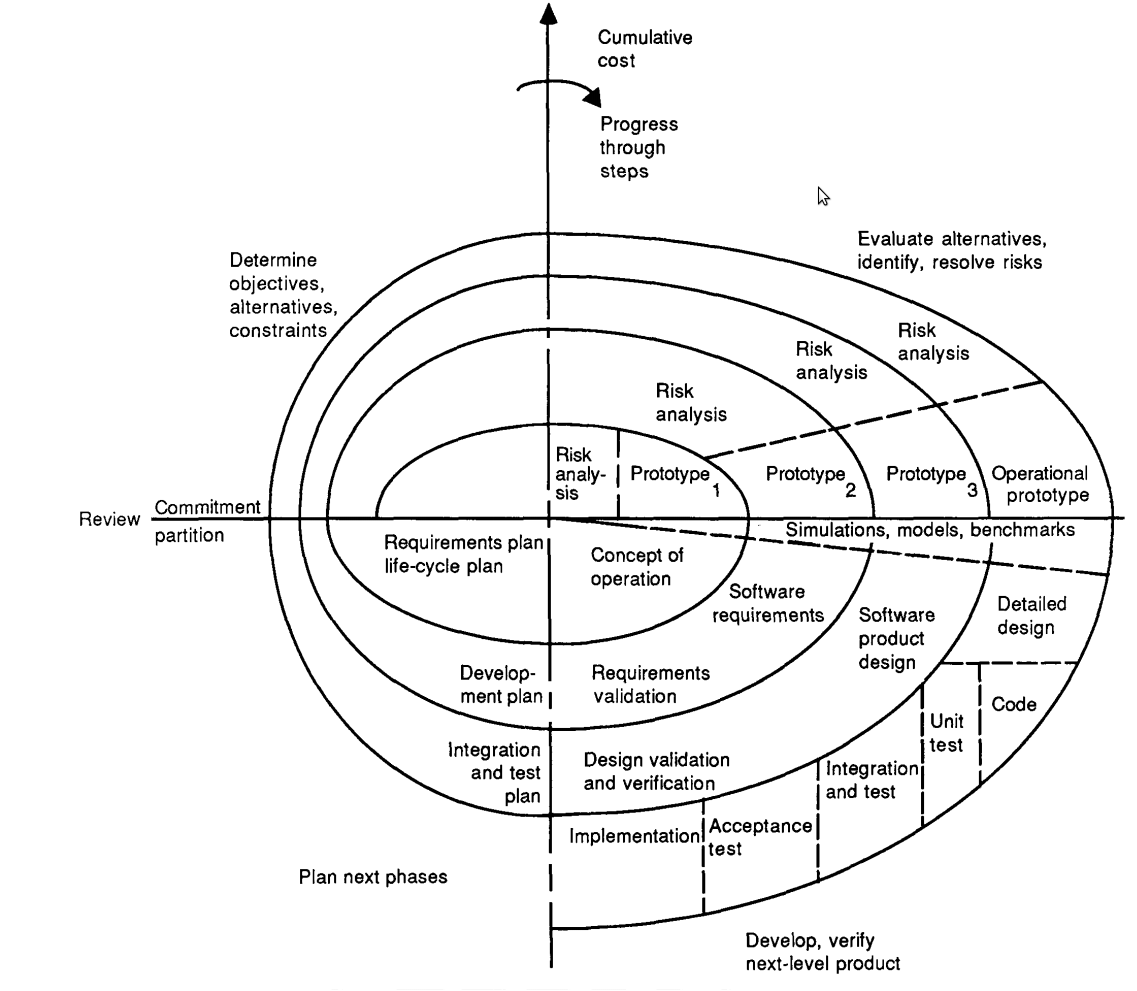
\includegraphics[width=\textwidth]{spiral}
\end{figure}

\subsection*{Suunnittelu ja analysointi}

Spiraalimallissa jokainen vaihe aloitetaan tunnistamalla:
\begin{itemize}
  \item laadittavien ohjelmisto-osien suorituskykyyn, toiminnallisuuteen sekä sopeutumiskykyyn liittyvät tavoitteet
  \item vaihtoehtoiset toteutustavat (ohjelmiston osto, ohjelmiston uudelleenkäyttö, vaihtoehtoiset ohjelmat)
  \item ohjelmiston eri vaihtoehdoille asettamien rajoitteet (rajapinnat, aikataulu, kustannukset)\cite{BOE88}.
\end{itemize}

\subsection*{Riskien tunnistaminen ja prototyyppi}

Seuraava askel on arvioida vaihtoehtoja suhteessa ohjelmiston tavoitteisiin ja rajoitteisiin. Usein tämä prosessi tunnistaa epävarmoja alueita, jotka ovat merkittäviä riskin lähteitä. Riskien löytyessä, seuraava askel pitää sisällään kustannustehokkaan strategian muotoilun riskien ratkaisemiseksi. Tähän voi liittyä prototyyppien valmistamista, simulointia, vertailuanalyysia, kyselylomakkeita, analyyttista mallinnusta, tai näiden yhdistelmiä sekä muita riskien ratkaisumenetelmiä\cite{BOE88}.

\subsection*{Suunnittelua ja ohjelmiston kehitystä}

Jos suorituskykyyn tai käyttöliittymään liittyvät riskit voimakkaasti hallitsevat ohjelman kehittämistä, seuraavassa vaiheessa kehityksellisesti (evolutionary), mahdollisimman vaivattomasti, määritellään ohjelmiston yleistä luonnetta, suunnitellaan seuraavan tason prototyyppiä ja kehitetään yksityiskohtaisempaa prototyyppiä riskien ratkaisemiseksi\cite{BOE88}.

Riskinhallinta huomioiden voidaan määritellä kiinnitettävä aika ja työmäärä toiminnan suunnitteluun (planning), asetuksien hallintaan (configuration management), laadun varmistukseen(quality assurance), muodolliseen todentamiseen (formal verification) ja testaukseen\cite{BOE88}.

\subsection*{Katselmus}

Spiraalimallin tärkeä ominaisuus on, että jokainen iteraatio päätetään katselmukseen tuotteeseen liittyvän henkilöstön tai organisaation kanssa\cite{BOE88}.

\subsection*{Testaus}

Barry Boehmin kuvaamassa spriraalimallissa yksikkö-, integraatio- ja hyväksymis\-testit ovat ohjelmiston kehityskaaren lopussa. Spriraalimallin riskiperustaisesta lähestymistavasta huolimatta, ohjelmiston kehitysprosessi sisältää riskejä. Kuten Winston Royce huomauttaa artikkelissaan ''Managing the development of large software systems'' lineaarisen prosessin riskeistä: testausvaiheessa ilmenee ongelmia, joita analysointi vaiheessa ei ollut mahdollista selvittää. Testauksen ollessa vasta kehityskaaren lopussa, ohjelmiston kehitysprosessi saattaa pitkittyä jos ohjelman korjaaminen vaatii mittavia rakennemuutoksia ja ohjelmiston uudelleen suunnittelua\cite{ROY70}.

\section{Ketterät kehitysmenetelmät}

Ketterät menetelmät (agile methods) ovat saavuttaneet suosiota ohjelmistotuotannossa. Usein iteraatiivisia, inkrementaalisia sekä kehityksellisiä (evolutionary) menetelmiä pidetään modernina ohjelmistokehityksenä, mikä on korvannut vesiputousmallin. Mutta näitä menetelmiä on käytetty vuosikymmeniä\cite{LAB03}.

Monet ohjelmistotuotantoprojektit  (esimerkiksi NASA:n Mercury- ja avaruussukkula-projektit) 1970- ja 1980-luvulla käyttivät iteraatiivisia ja inkrementaalisia menetelmiä.  Menetelmillä oli eroavaisuuksia iteraatioiden pituuksissa ja aikarajoitteiden käytössä (time-box). Joillakin oli merkittävä suunnittelu- ja vaatimusmäärittelyvaihe (big design up front), jota seurasi inkrementaalinen aikarajoitettu (time-box) kehitysvaihe. Toisilla oli enemmän kehityksellisempi ja palautteen ohjaama lähestymistapa\cite{LAB03}.

Eroavaisuuksista huolimatta, kaikilla lähestymistavoilla oli yhteistä välttää, lineaarisesta yksi vaihe kerrallaan etenevää, dokumenttiperustaista menetelmää\cite{LAB03}.

Lineaarisesti vaiheesta toiseen etenevän ohjelmistotuotantomenetelmä ei sovi erityisesti interaktiivisiin loppukäyttäjien sovelluksiin. Suunnitelmavetoiset standardit pakottavat dokumentoimaan yksityiskohtaisesti heikosti ymmärretyt käyttöliittymien vaatimukset\cite{BOE88}.

Tästä seurasi käyttökelvottoman ohjelmakoodin suunnittelua ja toteutusta. Lineaarisen ohjelmistotuotantomenetelmän vaiheet olivat tällaisille projekteille selvästi väärässä järjestyksessä. Erityisesti joillekin ohjelmistoille ei ole tarvetta yksityiskohtaiselle dokumentaatiolle ennen toteutusta\cite{BOE88}.

Seurauksena muuttuvista vaatimuksista useat ohjelmistoalan ihmiset ja organisaatiot kehittivät menetelmiä ja käytäntöjä, joille muutokset ovat hyväksyttyjä. Nämä uudet menetelmät toivottavat muutokset tervetulleiksi, ja ohjelmisto kehittyy uusiin vaatimuksiin ja muutoksiin mukautuen\cite{WIC03}. Perinteinen lähestymistapa perustui oletukselle, että aikaisella ja täydellisellä vaatimusmäärittelyllä voidaan pienentää kustannuksia vähentämällä muutoksia. Nykyään muutosten kieltäminen merkitsee reagoimattomuutta liiketoimintaympäristön kehitykselle\cite{HIC01}.

Menetelmiä kehitettiin useita ja eri maissa: 
\begin{itemize}
 \item Taipuisa järjestelmän kehitysmenetelmä (Dynamic Systems Development) Euroopassa
 \item toiminnallisuusvetoinen kehitysmenetelmä (Feature-Driven Development) Australiassa
 \item ja XP (Extreme Programming)\cite{BEC99}, Crystal\cite{COC05}, mukautuva ohjelmistokehitys (Adaptive Software Development) ja Scrum\cite{SCH09} Yhdysvalloissa\cite{WIC03}.
\end{itemize}

Helmikuussa 2001 17 menetelmien kehittäjää tapasi keskustellakseen kevyistä menetelmistä ja kokemuksiensa yhtäläisyyksistä. Huomatessaan, että heidän käytänteillään oli paljon yhteistä, ja että heidän prosessinsa tarjosivat keinoja saavuttaa merkityksellinen päämäärä: asiakkaan tyytyväisyys ja korkea laatu\cite{WIC03}. 

Osallistujat määrittelivät käytännöt ketteriksi menetelmiksi.
Osallistujat kirjoittivat ''Manifesto for Agile Software Development''-julistuksen, mikä kuvaa ketterän kehityksen perusarvoja:

\begin{itemize}
 \item Yksilöt ja vuorovaikutus ennen prosesseja ja työkaluja
 \item Toimiva ohjelmisto ennen kattavaa dokumentaatiota
 \item Asiakasyhteistyö ennen sopimusneuvotteluja
 \item Muutoksiin vastaaminen ennen suunnitelman seuraamista\cite{WIC03}.
\end{itemize}

Ohjelmistotuotannon parissa työskentelevät huomasivat, että ohjelmistoinsinööritieteet erosivat huomattavasti muista insinööritieteistä. Autojen kokoaminen on määriteltävä prosessi. Insinöörit voivat suunnitella prosessin, määritellä kokoonpanojärjestyksen sekä työntekijöiden, koneiden tai robottien toimenpiteet\cite{WIC03}. Ohjelmistotuotantoprojektit ovat luonteeltaan empiirisiä prosesseja, joiden lopputuloksena syntyy uusia tuotteita. Projektin aikana on oleellista oppia prosessin edetessä ja mukautua, eikä määritellä kaikkea alussa kattavasti. Empiirinen prosessi vaatii "tarkkaile ja mukaudu"-tyyppisen lähestymistavan. Lyhyet iteraatiot auttavat ketteriä menetelmiä mukautumaan ja muuttamaan ohjelmistoteollisuuden ennustamattomien vaatimuksien mukaan\cite{WIC03}.

\subsection{Extreme programming}

XP (Extreme Programming) vähentää ohjelmiston vaatimusten muuttumisen kustannuksia tekemällä koko kehityskaaren aikaisia toimintoja jatkuvasti ohjelmistokehityksen aikana. Perinteisen ohjelmistotuotantoprosessin sijaan suunnitellaan, analysoidaan ja muotoillaan rakennetta vähän kerrallaan\cite{BEC99}.

Asiakas valitsee seuraavaan iteraatioon eniten arvoa tuottavat tarinat (story). Ohjelmoijat jakavat tarinat pieniksi tehtäviksi (task). Ohjelmoijat muuttavat tehtävät joukoksi testejä, jotka osoittavat tehtävän valmistuneen. Parin kanssa työskentelemällä ohjelmoija ajaa testejä ja kehittää samalla mahdollisimman yksinkertaista suunnitelmaa tehtävän ratkaisemiseksi\cite{BEC99}.

\subsection*{Julkaisu}

Asiakas valitsee mahdollisimman pienen määrän toiminnallisuuksia, jotka tuottavat eniten arvoa ohjelmistolle ja toimivat julkaistavana ohjelmistona. Määrätyt toiminnallisuudet toteutetaan ensin ja ohjelmisto julkaistaan. Asiakkaan on priorisoitava tärkeimmät toiminnallisuudet, jotka hän haluaa ohjelmistoon toteutettavan ensimmäisenä\cite{BEC99}. 

Suunnitteluprosessin (planning game) aikana tiimi määrittää toiminnallisuuksille hinnan - aika-arvion. Arvio saadaan jakamalla tiimin tekemät toiminnallisuudet toteutukseen vaaditulla aikayksiköllä. Julkaisun budjetti lasketaan toivottujen toiminnallisuuksien aika-arvioiden perusteella. Asiakas voi valita halutut toiminnallisuudet ja pyytää tiimiä laskemaan julkaisupäivän. Tai asiakas voi valita julkaisupäivän ja valita tarinoita julkaisuun kunnes budjetti täyttyy.\cite{BEC99}.

Ohjelmisto laitetaan tuotantoon nopealla aikataululla. Uusia versioita julkaistaan usein - kuukausittain tai jopa päivittäin. Uutta ohjelmakoodia integroidaan nykyiseen ohjelmistoon jopa muutaman tunnin välein (continuos integration). Integroidessa uutta koodia koko järjestelmä rakennetaan alusta uudestaan ja kaikki testit ovat läpäistävä, tai kaikki muutokset hylätään\cite{BEC99}.  


\subsection*{Iteraatio}

Jokaisen iteraation tarkoituksena on lisätä ohjelmistoon uusia toiminnallisuuksia, jotka ovat testattuja ja valmiita. Prosessi alussa asiakas ja ohjelmoijat suunnittelevat joukon tarinoita, jotka toteutetaan ohjelmistoon. Iteraatiota suunniteltaessa asiakas valitsee eniten arvoa tuottavat toiminnallisuudet. Tiimi pilkkoo toiminnallisuudet pienemmiksi tehtäviksi. Tehtävät ovat toiminnallisuuden osia, jotka yksi ohjelmoija voi toteuttaa muutamassa päivässä. Asiakas laatii hyväksymistestit tarinalle (functional test) ja tiimi toteuttaa vaaditun toiminnallisuuden. Iteraation lopussa testit ajetaan hyväksytysti ja prosessi on valmis seuraavaan iteraatioon\cite{BEC99}.

\subsection*{Tarina}

Ohjelmistoa suunniteltaessa on päätettävä mitä ohjelmalla tehdään ja mitä sen on tehtävä ensin. Analyysin perusteella muodostetaan tarina (story) - käyttötapaus - joka voidaan kirjoittaa pienelle kortille. Jokainen tarina on oltava arvoa tuottava toiminnallisuus, joka on testattavissa ja arvioitavissa\cite{BEC99}.

\subsection*{Tehtävä}

Toteuttaakseen tehtävän (task) ohjelmoijat työskentelevät pareittain, jos ilmenee kysymyksiä toteutuksesta tai toiminnallisuuden laajuudesta pari keskustelee hetken jatkuvasti paikalla olevan asiakkaan (on-site customer) kanssa. Pari tiivistää toiminnallisuuden testitapauksiksi, jotka ovat ajettavissa ennen kuin tehtävä on valmis. Testit luovat pohjan tuotettavalle ohjelmakoodille ja pari pyrkii mahdollisimman yksinkertaiseen tapaan ratkaista testitapaukset. Kun ohjelmakoodi läpäisee testit, ohjelmoijat suunnittelevat rakennetta uudelleen (refactoring), jos on tarvetta\cite{BEC99}.     

\subsection*{Testit}

XP:ssä testausta painotetaan paljon. Kaikki ohjelmoijat testaavat tehdessään tuotantokoodia. Ohjelmoijat liittävät uudet testitapaukset ja tuotetut toiminnallisuudet ohjelmistoon. Tämä varmistaa jatkuvan integraation (continuos integration) ja vaakaan rakennusprosessin\cite{FOW01a}.

Ohjelmoijat kirjoittavat testin toiminnallisuudelle ennen tuotantokoodia. Testit ovat jatkuvasti osana ohjelmistoa. Iteraation alussa asiakas päättää miten vakuuttaa, että uusi tarina on lisätty onnistuneesti ohjelmistoon. Hänen päätökset, uuden toiminnallisuuden toimivuudesta, muutetaan koko järjestelmän laajuisiksi testeiksi. Testit takaavat ohjelmoijille ja sidosryhmille, että ohjelmisto toimii ja täyttää odotetut vaatimukset. Testit ovat ajettavissa koko ohjelmiston kehityskaaren ajan, mikä takaa ohjelmiston toimivuuden, kun lisätään uusia toiminnallisuuksia tai ohjelmakoodin rakennetta muutetaan\cite{BEC99}.

Winston Royce kirjoitti artikkelissaan ''Managing the development of large software systems'', että ohjelmoijan ei tule testata kirjoittamaansa ohjelmakoodia. Royce arvioi, että useimmat virheet ovat ilmiselviä ja ovat löydettävissä ohjelmakoodia visuaalisesti tarkastelemalla\cite{ROY70}. XP:ssä tätä ongelmaa on lähestytty työskentelemällä jatkuvasti pareittain\cite{BEC99}. 


\subsection{Scrum}

Scrum lähestyy ohjelmistotuotantoprojektin monimutkaisuutta joukolla yksinkertaisia käytänteitä ja sääntöjä. Scrum on tarkasteleva, mukautuva ja empiirinen prosessi. Scrum perustaa kaiken käytännön iteratiiviselle ja inkrementaaliselle prosessille. Jokaisen iteraation tulos on ohjelmistotuotteen inkrementaalinen edistyminen. Iteraatioita vie eteenpäin lista vaatimuksista\cite{SCH09}. 

Iteraation alussa tiimi selvittää mitä sen on tehtävä. Tiimi harkitsee saatavilla olevia teknologioita, arvio omia taitojaan ja kykyjään. Tiimi yhdessä päättää miten uusi toiminnallisuus toteutetaan, mukautuen vaikeuksiin ja yllätyksiin. Tiimi työskentelee rauhassa parhaan kykynsä mukaan lopun iteraation ajan. Iteraation lopussa tiimi esittelee toiminnallisuuden sidosryhmille, jotka tarkastelevat toiminnallisuutta ja tarvittavat muutokset voidaan tehdä riittävän ajoissa\cite{SCH09}.

\subsection*{Scrum roolit}

Scrum määrittää kolme eri roolia: tuoteomistaja (Product owner), kehittäjätiimi (Team) ja scrummaster (Scrum master). Kaikki projektin hallinnolliset vastuut on jaettu näiden roolien kesken. Tuoteomistajan vastuu on esitellä sidosryhmän, projektin lopulliselle tuotteelle asetettavat, vaatimukset. Tuoteomistaja laatii alustavan vaatimusmäärittelyn, sijoitettavalle pääomalle asetettavat tavoitteet (ROI) ja julkaisu suunnitelmat (relese plans). Tuoteomistaja vastaa, että vaatimuslistan (Product backlog) eniten arvoa tuottavat toiminnallisuudet toteutetaan ensin. Tuoteomistaja priorisoi vaatimuslistan toiminnallisuuksia. Näin seuraavassa iteraatiossa lisätään eniten arvoa tuottavat toiminnallisuudet ensin\cite{SCH09}. 

Tiimin vastuulla on toiminnallisuuksien kehittäminen. Tiimi on monipuolisesti eri alojen asiantuntemuksen omaamista ihmisistä koostuva ryhmä ja se on itse-organisoituva. Heidän tehtävä on vaatimuslistan toiminnallisuuksien lisääminen inkrementaalisesti iteraation aikana. Tiimi on yhdessä vastuussa jokaisen iteraation onnistumisesta. Scrummaster on vastuussa itse Scrum prosessista. Hänen tehtävänä on esitellä Scrumin periaatteet jokaiselle projektiin osallistuvalle, sekä toteuttaa Scrumia niin, että se sopii organisaation kulttuuriin ja toteuttaa odotetut hyödyt. Scrummaster valvoo, että jokainen toteuttaa ja seuraa Scrumin periaatteita\cite{SCH09}.

\subsection*{Tuotteen kehitysjono}

Tuoteomistajalla on olemassa tuotettavasta ohjelmistosta näkemys. Tuoteomistajan visio konkretisoituu listana vaatimuksista tuotteen kehitysjonona (product backlog). tuotteen kehitysjono on priorisoitu: toiminnallisuudet jotka tuottavat arvoa ovat ylimpänä listassa. Tuotteen kehitysjono on projektin lähtökohta ja sen sisältö, prioriteetit ja ryhmittely julkaisuihin yleensä muuttuvat projektin käynnistyttyä. Muutokset tuotteen kehitysjonossa heijastavat muuttuvaa liiketoimintaympäristöä ja tiiimin nopeutta toteuttaa toiminnallisuuksia\cite{SCH09}.

\subsection*{Sprintin tehtävälista}

Sprintin tehtävälista (Sprint backlog) sisältää tiimin määrittelevät tehtävät, joita tiimi toteuttaa. Tehtävät ovat tuotteen kehitysjonosta sprinttiin valittuja toiminnallisuuksia, jotka tiimi on pilkkonut pienempiin osiin. Jokainen tehtävä tulisi olla noin 4-16 tunnin pituinen ohjelmointitehtävä. Ainoastaan tiimi voi muuttaa sprintin tehtävälistaa. Sprintin tehtävälista on läpinäkyvä, reaaliaikainen kuva, mitä tiimi pyrkii saavuttamaan kyseessä olevassa sprintissä. Tehtävän yhteydessä on kirjattu arvio ajasta, jonka kyseessä olevaan tehtävään on arvioitu kuluvan, ja henkilö kuka on vastuussa kyseisestä tehtävästä\cite{SCH09}.

\subsection*{Sprintti}

Kaikki työ tehdään 30 päivän iteraatioissa (Sprint). Jokainen sprintti alkaa iteraation suunnittelupalaverilla (Sprint planning meeting), jossa tuoteomistaja ja tiimi yhteistyössä päättävät mitä toteutetaan. Valitsemalla tuotteen kehitysjonosta korkeimman prioriteetin toiminnallisuudet tuoteomistaja kertoo mitä hän toivoo ja tiimi selvittää miten paljon toivomuksista he voivat muuttaa toiminnallisuuksiksi seuraavassa sprintissä\cite{SCH09}.

Joka päivä tiimi kokoontuu 15 minuutin tapaamiseen - päiväpalaveriin (Daily Scrum). Jokainen tiimin jäsen vastaa kolmeen kysymykseen: Mitä olen tehnyt viimeisen tapaamisen jälkeen? Mitä ajattelin tehdä seuraavaksi? Mikä estää minua saavuttamasta tavoitteitani? Tapaamisen tarkoituksena on synkronoida tiimin työ päivittäin ja sopia tapaamisista, joita tiimi tarvitsee edetäkseen työssään\cite{SCH09}.

Iteraation lopussa pidetään sprinttikatselmus (Sprint review meeting), jossa tiimi esittelee tuoteomistajalle ja muille sidosryhmille, jotka haluavat osallistua, mitä tiimi on kehittänyt iteraation aikana. Tapaamisen tarkoituksena on tuoda ihmiset yhteen, esitellä ohjelmiston toiminnallisuudet ja auttaa osallistujia yhdessä päättämään, mitä tiimin tulisi seuraavaksi tehdä\cite{SCH09}. 

Sprinttikatselmuksen jälkeen ja ennen seuraavan sprintin suunnittelupalaveria, scrummaster ja tiimi pitää sprintin retrospektiivin (Sprint retrospective meeting). Scrummaster rohkaisee tiimiä kertaamaan kehitysprosessiaan, tehdäkseen siitä tehokkaampaa ja nautittavampaa seuraavaan iteraatioon\cite{SCH09}.

Yhdessä sprintin suunnittelupalaveri, päiväpalaveri, sprinttikatselmus ja sprintin retrospektiivi muodostavat scrumista empiirisen, tarkastelevan ja sopeutuvan projektinhallintakehyksen\cite{SCH09}.

\subsection*{Julkaisu}
Scrumissa on kaikkien tiimin jäsenten oltava selvillä määritelmästä ''valmis toiminnallisuus''. Scrum vaatii tuotteeseen lisättävän toiminnallisuuden olevan kattavasti testattu, rakenteeltaan hyvin suunniteltua ja kirjoitettua ohjelmakoodia, ja toiminnallisuus on oltava dokumentoituna operaation käyttäjälle. Tuotteella saattaa olla lisäksi muita vaatimuksia standardien tai käytänteiden muodossa\cite{SCH09}.

\section{Ohjelmiston laatu}

\subsection{Ohjelmiston suunnittelu}

Suunnitelmavetoisissa menetelmissä ohjelmistosuunnittelijat suunnittelevat etukäteen isoa kokonaiskuvaa koko järjestelmästä. Suunnittelijoiden ei tarvitse miettiä jokaista pientä yksityiskohtaa, koska suunnittelutekniikat, kuten UML (unified modeling language) antavat mahdollisuuden työskennellä abstraktimmalla tasolla. Suunnittelijoiden ei tarvitse ottaa huomioon käytännön ohjelmointia ja sen aiheuttamaa entropiaa. Suunnittelijan on kuitenkin mahdotonta ottaa huomioon kaikkia yksityiskohtia, mitä ohjelmoija joutuu ratkaisemaan yksityiskohtaisemmalla tasolla\cite{FOW01b}.

Kehityksellinen suunnittelu, jossa suunnitelma on ainoastaan perättäisiä erillisiä taktisia päätöksiä, johtaa tavallisesti vaikeasti muutettavaan ohjelmakoodiin. Voidaan sanoa ettei tällainen ole suunniteltua ohjelmistokehitystä. Tai ainakin tällainen menettely johtaa huonoon ohjelmiston rakenteeseen. Suunnitelman heikentyessä vaikeutuu kyky tehdä muutoksia tehokkaasti\cite{FOW01b}. 

Ohjelmistoprojektin edetessä ja entropian lisääntyessä ohjelmiston rakenne huononee. Tämä ei ainoastaan vaikeuta ohjelmiston muuttamista, vaan lisää virheiden määrää. Ja virheiden löytäminen sekä niiden poistaminen ohjelmistosta vaikeutuu. Tällainen on ''ohjelmoi ja korjaa''-menetelmän tyypillinen ongelma: ohjelmistovirheiden korjaaminen on eksponentiaalisesti kalliimpaa projektin edetessä\cite{FOW01b}.

Winston Roycen vesiputousmalli\cite{ROY70} ja Barry Boehmin spriraalimalli\cite{BOE88} perustavat ohjelmistokehityksen vahvasti dokumentti- ja suunnitelmavetoisille prosessille, jossa tuotettavaa ohjelmistoa ja ongelma-aluetta pyritään lähestymään analyysin, vaatimusmäärittelyn sekä suunnittelun kautta. Molemmissa malleissa ratkaisuksi ohjelmistotuotannon ongelmiin esitetään prototyypin valmistamista, mitä testaamalla ilmeneviin ongelmiin voidaan reagoida mahdollisimman aikaisin.

Royce ehdottaa vesiputousmallissa, että prototyypin kehityksen aikataulu on kolmannes varsinaisen tuotteen kehitykseen vaaditusta ajasta\cite{ROY70}. Boehm ei määritellyt spiraalimallissa iteraatioiden pituutta suhteessa ohjelmistokehitykseen vaadittuun aikaan. Mutta spiraalimallissa Boehm painottaa vahvasti prototyypin osuutta ohjelmiston kehityskaaren aikana. Varhainen prototyyppi tarjoaa ohjelmiston testattavaksi, jotta virheitä voidaan löytää aikaisessa vaiheessa. Asiakkaan kanssa tehdyssä katselmuksessa saadaan prototyypistä palautetta seuraavan iteraation prototyyppiin\cite{BOE88}.

Erityisesti Royce painotti artikkelissaan ''Managing the development of large software systems'' dokumentoinnin tärkeyttä\cite{ROY70}. Suunnitelmavetoisten prosessien mukautuminen muuttuviin muutoksiin vaikeutuu kattavan dokumentoinnin takia. Nopeasti muuttuvat vaatimukset tekevät dokumenteista vanhentuneita, ja niiden päivittäminen vaati aikaa. Turhien kaavioiden piirtämiseen kuluu kalliita resursseja, kun suunnitelmat muuttuvat. Kaaviot vanhentuvat ja käyvät tarpeettomiksi\cite{FOW01b}.

Edellä kuvatuissa ketterissä ohjelmistotuotannon menetelmissä on yhteistä pyrkimys formaalilla tavalla määritellä ohjelmistotuotannon prosessi, jolla voidaan välttää ''ohjelmoi ja korjaa''-menetelmän ja suunnitelmavetoisten prosessien ongelmat. Suunnitelmavetoisissa menetelmissä on pyritty tehostamaan vaatimusmäärittelyprosessia, jotta vaatimukset voidaan kattavasti määritellä ja ettei muutoksille ole tarvetta ohjelmistokehityksen edetessä. Monia odottamattomia muutoksia vaatimuksissa tapahtuu kuitenkin koska liiketoimintaympäristö muuttuu\cite{FOW01b}.

Ketterien menetelmien prosesseissa suunnittelussa painotetaan joustavuutta, jotta suunnitelmaa voidaan helposti muuttaa kun vaatimukset muuttuvat. XP:ssä suunnitelmien ja kaavioiden merkitys on vähäinen: UML kaavioita tulisi käyttää, jos niistä on hyötyä. Äärimäiset XP:n toteuttajat eivät käytä UML-kaavioita lainkaan\cite{FOW01b}. Kaavioiden merkitys on tarjota yhteydenpitoa. Tehokkaan yhteydenpidon takaamiseksi on piirrettävään kaavioon valittava tärkeät asiat ja vältettävä vähemmän tärkeitä. Vain merkitykselliset luokat sekä niiden tärkeimmät attribuutit ja operaatiot tulee kuvata UML-kaavioon\cite{FOW01b}.

Tehtyä kaaviota on pidettävä luonnoksena ei valmiina suunnitelmana. Ohjelmoinnin edetessä usein selviää, että jotkin suunnitelman osa-alueet ovat vääriä. Usein ongelma ei ole suunnitelmien muuttamisessa. Ongelmana on, että usein ihmiset ajattelevat suunnitelman olevan valmis, eivätkä vie ohjelmoidessa saatua tietoa takaisin suunnitelmaan\cite{FOW01b}. 

Suunnitelmien muututtua ei kaaviota tarvitse välttämättä muuttaa. On täysin perusteltua piirtää kaaviota ymmärtääkseen ohjelmiston rakennetta ja heittää kaaviot toteutuksen jälkeen pois. Kaavioiden piirtämisen hyöty on jo saavutettu rakenteen suunnittelulla ja sen ymmärtämisellä. Kaavioiden ei tule olla pysyviä suunnitelman osia\cite{FOW01b}.

Ohjelmoinnin aikaista dokumentointia voidaan muuttuviin vaatimuksiin ja suunnitelmiin sopeuttaa seuraavasti:

\begin{itemize}
 \item Käytetään vain kaavioita, joita voidaan pitää ajan tasalla helposti 
 \item Laitetaan kaaviot paikkaan, jossa ne ovat helposti nähtävillä
 \item Kannustetaan ihmisiä muuttamaan kaavioita
 \item Heitetään pois kaaviot joita ihmiset eivät käytä\cite{FOW01b}.
\end{itemize}

Usein UML-kaavioita käytetään välittämään tietoa eri ryhmien välillä. XP:n näkökulmasta UML-kaaviot ovat tarinoita muiden joukossa, joiden arvon määrää asiakas. UML-kaaviot ovat hyödyllisiä vain jos ne auttavat viestinnässä. Ohjelmakoodin varasto (repository) on yksityiskohtaisen tiedon lähde ja kaaviot koostavat ja korostavat tärkeitä asioita\cite{FOW01b}.    


\subsection{Ohjelmiston testaus}


\subsection{Pariohjelmointi}

Pariohjelmoinnissa kaksi ohjelmoijaa yhdessä työstävät yhtä ohjelmakoodia, algoritmia tai suunnitelmaa. Toinen parista, ajaja, ohjelmoi ja toinen aktiivisesti tarkkailee ajajan työtä, etsien virheitä, miettien vaihtoehtoja, tutkien lähteitä ja miettien strategisia toteutustapoja. Parit vaihtavat roolejaan jaksoittain. Molemmat ovat tasavertaisia ja aktiivisia osallistujia\cite{WIL00}.

Pariohjelmoinnin kustannukset ovat oleellinen asia. Jos kustannukset ovat suuret, johtajat eivät salli pariohjelmointia. Epäluuloiset olettavat, että pariohjelmoinnin sisällyttäminen ohjelmistotuotantoon kaksinkertaistaa kustannukset jos henkilöstömäärää on lisättävä samassa suhteessa. Tutkimukset kuitenkin osoittavat, että pareittain työskentelevät tiimit suoriutuvat tehokkaammin kuin yksittäiset ohjelmoijat\cite{NOS98}\cite{WIL00}.

Pareittain työskentelevät tuottavat luettavampaa ohjelmakoodia ja toimivampia ratkaisuja kuin yksin toimivat ohjelmoijat. Ryhmissä toimivat ratkaisevat ongelmia keskimäärin nopeammin kuin yksilöt. Lisäksi pareittain toimivat ilmaisevat korkeampaa luottamusta ratkaisuunsa ja kokevat nauttivansa prosessista enemmän kuin yksin toimivat ohjelmoijat\cite{NOS98}.   

Pariohjelmointi tuottaa erityisesti parempaa suunnittelua ja analyysia kuin yksilölliset ohjelmoijat. Pari harkitsee huomattavasti enemmän vaihtoehtoja ja yhtyvät nopeasti toteutettavaan ratkaisuun. Ideoiden vaihto parin välillä merkittävästi vähentää huonon rakennesuunnitelman todennäköisyyttä.  Yhdessä työskentelemällä pari voi toteuttaa tehtäviä, jotka voivat olla liian haastavia yhdelle. Parityöskentely pakottaa osallistujia keskittymään täysin haasteena olevaan tehtävään\cite{WIL00}.

Vuonna 1998 John Nosek teki tutkimuksen, jossa kokeneet ohjelmoijat työskentelivät haastavien, omalle organisaatiolleen tärkeiden, tehtävien parissa omassa työskentely-ympäristössään. Kukaan osallistujista ei ollut työskennellyt annetun tehtävän kaltaisen ongelman parissa aikaisemmin. Annetun tehtävän kaltaista ongelmaa pidettiin organisaatiolle menestykselle tärkeänä ja niin vaativana, että yleensä tehtäviin palkattiin ulkopuolisia konsultteja\cite{NOS98}.

Koehenkilöt valittiin satunnaisesti työskentelemään pareittain testiryhmään ja yksilöinä kontrolliryhmään.
Ryhmiltä tehtäviin kulunut aika mitattiin. Ratkaisuista pisteytettiin luettavuus väliltä 0-2. Lukuarvo 0 tarkoitti lukukelvotonta ratkaisua ja 2 täysin luettavissa olevaa ratkaisua. Ratkaisun toimivuus pisteytettiin väliltä 0-6. Lukuarvo 0 merkitsi, että ratkaisu ei saavuttanut annettua tehtävää lainkaan. Täysin toimiva ratkaisu pisteytettiin arvolla 6. Kokonaispistemäärän maksimiarvo oli 8, joka oli luettavuuden ja toimivuuden summa\cite{NOS98}.

Pareittain työskentelevät saivat keskimäärin kokonaispistemääräksi 7,6 ja aikaa kului 30,2 minuuttia. Vertailuryhmän keskimääräinen kokonaispistemäärä oli 5,6 ja tehtävään aikaa kului 42,6 minuuttia\cite{NOS98}.

Vuonna 1999 Utahin yliopiston tietojenkäsittelytieteen opiskelijat osallistuivat tutkimukseen. Opiskelijat jaettiin kahteen ryhmään. Kolmetoista opiskelijaa muodosti kontrolliryhmän, jossa opiskelijat työskentelivät itsenäisesti kaikissa annetuissa tehtävissä. 28 opiskelijaa muodosti testiryhmän, jossa opiskelijat muodostivat kahden hengen ryhmän. Kokeilu vertaili tehtävistä suoriutumiseen vaadittua aikaa, tuottavuutta ja suoritettujen tehtävien laatua ryhmien välillä. Puolueeton assistentti suoritti automaattiset testit arvioidakseen ohjelmointityön laatua\cite{WIL00}.

Monet opiskelijat olivat epäluuloisia pariohjelmoinnin hyödyistä: he pohtivat paljonko ylimääräistä kommunikaatiota vaaditaan, miten he sopeutuvat toistensa työskentelytapoihin, ohjelmointityyliin ja miten heidän egonsa vaikuttavat työskentelyyn, sekä miten erimielisiä he ovat tehtävien toteutuksista. Tosiasiassa ohjelmoijat käyvät läpi siirtymäajan yksinäisestä työskentelystä yhteisölliseen työskentelytapaan. Siirtymäajan kuluessa he oppivat sopeuttamaan toimintojaan käyttämään hyväksi vahvuuksiaan ja välttämään heikkouksia. Tuloksena ryhmän tuottavuus ylittää ryhmän yksilöiden tuottavuuden summan.\cite{WIL00}.

Nosekin tekemässä tutkimuksessa pareittain työskentelevät käyttivät, työskennellessään rinnakkain, yhteensä 60\% enemmän ohjelmointiaikaa kuin yksin työskentelevät\cite{NOS98}. Utahin opiskelijoille tehdyssä tutkimuksessa saatiin samankaltaisia tuloksia: keskimäärin pareittain työskenteleviltä vaati yhteensä 60\% enemmän ohjelmointiaikaa annetusta tehtävästä suoriutumiseen\cite{WIL00}.

Siirtymäajan jälkeen pareittain työskentelevät opiskelijat paransivat tuloksiaan. Pareittain työskenteleviltä vaadittu ohjelmointiaika oli enää 15\% suurempi kuin yksin työskentelevillä\cite{WIL00}.

Tutkimustulos pariohjelmoinnista\cite{WIL00}:

\subsection*{Läpäistyt testitapaukset prosentteina}
\begin{center}
    \begin{tabular}{ | l | l | p{5cm} |}
    \hline
    Tehtävä & Yksin työskentelevät & Pareittain työskentelevät \\ \hline
    Ohjelma 1 & 73,4 & 86,4 \\ \hline
    Ohjelma 2 & 78,1 & 88,6 \\ \hline
    Ohjelma 3 & 70,4 & 87,1 \\ \hline
    Ohjelma 4 & 78,1 & 94,4 \\ \hline
    \end{tabular}
\end{center}


Laurie Williamsin, Ward Cunninghamin ja Ron Jeffriesin haastattelemat ohjelmoijat sanoivat, että pareittain analysointi ja suunnittelu on merkittävämpää kuin toiminnallisuuden toteuttaminen. Ohjelmoijat usein toteuttavat yksilöllisesti rutiinitehtäviä ja yksinkertaisia ohjelmakoodeja. Tällaisten tehtävien toteuttaminen yksilöllisesti tehtynä tehokkaampaa\cite{WIL00}.

nosek\cite{NOS98}

cockburn\cite{COC00a}

\section{Johtopäätökset}


% --- Back matter ---
%
% bibtex is used to generate the bibliography. The babplain style
% will generate numeric references (e.g. [1]) appropriate for theoretical
% computer science. If you need alphanumeric references (e.g [Tur90]), use
%
% \bibliographystyle{babalpha}
%
% instead.

\bibliographystyle{babplain}
\bibliography{references-fi}


\end{document}
